\documentclass[11pt, letterpaper]{article}
\usepackage[letterpaper]{geometry}
\usepackage[hidelinks]{hyperref}
\usepackage{color}
\usepackage{subfig}
\usepackage[labelsep=period]{caption}
\usepackage{multirow}
\usepackage{adjustbox}
\usepackage[procnames]{listings}
\usepackage{epstopdf}
\DeclareGraphicsRule{.eps}{pdf}{.pdf}{`epstopdf #1}
\DeclareGraphicsExtensions{.pdf,.jpg,.jpeg,.png,.eps}

\definecolor{keywords}{RGB}{255,0,90}
\definecolor{comments}{RGB}{0,0,113}
\definecolor{red}{RGB}{160,0,0}
\definecolor{green}{RGB}{0,150,0}
\definecolor{mygray}{rgb}{0.5,0.5,0.5}
\usepackage{framed}
\lstset{language=Python, 
	    aboveskip=0.2ex,
	    belowskip=1ex,
        basicstyle=\ttfamily\small, 
        keywordstyle=\color{keywords},
        commentstyle=\color{comments},
        stringstyle=\color{red},
        keepspaces=true,
        frame=none,
        framesep=15pt,
        numbers=left,
        numbersep=12pt,
        numberstyle=\tiny\color{mygray},
        stepnumber=5,
		columns=flexible,
        showstringspaces=false,
        identifierstyle=\color{green},
        tabsize=2,
        xleftmargin=0.75cm,
        xrightmargin=0.95cm,
        procnamekeys={def,class}}

\captionsetup{belowskip=12pt}

\title{SWMM 5.1 Co-simulation Toolbox - User's Manual}
\author{Gerardo Andrés Riaño Briceño}

\begin{document}
\topskip0pt
\vspace*{\fill}
   \begin{center}
      \Large\textbf{SWMM 5.1 Co-simulation Toolbox - User's Manual}\\
      \small\textit{Universidad de los Andes - Department of Electrical and Electronic Engineering}
   \end{center}
\vspace*{\fill}
\pagebreak

\tableofcontents
\pagebreak


\setcounter{secnumdepth}{1}
\section{Introduction}
\setlength\parindent{0pt}
SWMM is an open source platform that is used for planning, analysis and design of related to stormwater runoff, combined and sanitary sewers, and other drainage systems in urban areas. Its mode of operation is to display an interface where a network can be modelled, using objects such as conduits, storage units, subcatchments, among others. The user sets attributes for each element in the network and then executes the calculation module of SWMM. 
\setlength\parindent{12pt}

Due to the changes that the design of sewer systems is suffering today, because of the inclusion of actuators, control rules, and optimal design, SWMM has become a limited tool; despite of its rule-based control module. However, it has a big potential being an open source software. Thanks to this, it is possible to enhance its functionality in order to include new methods that allow its users to simulate optimization and control processes. 

Consequently, a new toolbox for SWMM 5.1 has been developed, bringing new functionality to the program, as it was described before. This toolbox works as a co-simulation engine that retrieves information from SWMM during the simulation and allows to modify initial conditions, and attributes like an orifice/valve setting or the maximum volume of an storage unit.

Furthermore, in order to make this tool scalable and multidisciplinary, it has been developed for three programming languages: Python, Matlab and LabVIEW. The syntax for each tool is very similar, so it is easy to migrate from one to another depending on the type of project that is wanted to be developed. It is worth to say that this toolbox requires a little effort to be learnt if the user has worked with SWMM before. Nevertheless, some knowledge of the programming language is required. \\

That said, this document will cover six main topics that are described below. 
\begin{enumerate}
\item \emph{How does SWMM work?} - The main goal of this section is to clarify doubts related to SWMM file processing and explain, with a simplistic perspective, the calculation algorithm of SWMM; which is necessary to understand how the toolbox functions work, and how to use them for a co-simulation project.
\item \emph{How does the Toolbox work?} - General description of the Toolbox.
\item \emph{Co-simulation functions and constants} - Deep explanation of each of the functions and constants included in the toolbox.
\item \emph{Example running a single simulation.} - the example is developed for the three programming languages in order to compare the ways to declare a function in each one.
\item \emph{Example running $n$ simulations.}
\end{enumerate}
\pagebreak

\section{How does SWMM work?}
\setlength\parindent{0pt}

For the purpose of this manual, the complete explanation of the computational methods and the base model used by SWMM is not going to be explained; it can be checked in the SWMM 5 User's Manual which is available on the \textcolor{blue}{\href{http://www.epa.gov/nrmrl/wswrd/wq/models/swmm/}{SWMM Website}}. However, it is important to note that SWMM is a phisically based, discrete-time simulation model that employs principles of conservation of mass, energy and momentum \cite{•}. As a discrete-time tool its algorithm finds $n$ solutions, for the flow routing problem, in $n$ time intervals for a time window and initial conditions defined by the user. With that in mind, it is possible to understant now how SWMM makes its calculations checking the whole process; there are seven subprocesses which make up the  simulation algorithm as it is shown in Figure \ref{fig:run_simulation}.
\newline
\newline
\begin{figure}[ht!]
\begin{center}
\includegraphics[width=8.5cm]{figs/flow_chart}
\caption{Algorithm to run a simulation in SWMM.}
\label{fig:run_simulation}
\end{center}
\end{figure}

\begin{enumerate}
	\item Open SWMM files: SWMM opens three files along the simulation, the input file (.inp) that contains all the information about the model, the report file (.rpt) which contains a status report of the results of a run and the output file (.out) that is a binary file with the numerical results of a succesfull run.
	\item Start Simulation: the internal parameters of the program are initialized.
	\item Run Step: advances the simulation by one routing time step.
	\item End Subprocesses: all the computing systems and subprocesses of SWMM are ended.
	\item Calculate Mass Balance Error: at the end of a simulation SWMM calculates three errors based on the mass conservation principle, the runoff error, the flow routing error and the quality routing error.
	\item Write Report: SWMM writes the information for the output and report files.
	\item Close SWMM: the files used by SWMM are closed. The simulation is over.
\end{enumerate}


\section{How does the Toolbox work?}

This toolbox has been created as an additional module of the SWMM computational engine in order to preserve the code integrity. It has been compiled as a DLL, so it can be compatible with C-based programming languages. Additionally, some of the DLL functions that were created by the US-EPA were reused. Taking this into consideration, in order to enhance the toolbox functionality, following the style that has been used so far, you can download the original code of SWMM from the \textcolor{blue}{\href{http://www.epa.gov/nrmrl/wswrd/wq/models/swmm/}{SWMM Website}} and the toolbox C files from the \textcolor{blue}{\href{https://bitbucket.org/swmmtoolbox001}{Toolbox Repository}}.

\setlength\parindent{12pt}
So far only three new functions have been developed. These can be used for two different kinds of projects: running a SWMM simulation modifying the percentage of openning of an orifice and running several SWMM simulations in series, retrieving information and modifying initial conditions. At the end of this document, there are two examples that explain better what have been stated before.


\section{Co-simulation functions and constants}

The toolbox is composed of several functions that can reproduce a SWMM simulation with control actions and optimal model attributes. It also has useful constants that simplify the code development process. In the tables below both, general functions and constants, are described deeply.

Nevertheless, some of the return variables of the functions vary depending on the programming language. For instance, the "Run step" function for the Python Toolbox returns nothing, it just advances the simulation by one step, while the same function for the Matlab Toolbox returns the value of the current hour of simulation. This variations are explained better in the next section, where the differences between Toolboxes, secondary functions, and instantiation of methods are explained better.


\begin{center}
\begin{table}
\caption {Functions and their parameters with descriptions.} \label{tab:functions}  
\def\arraystretch{1.3}% 
\begin{adjustbox}{width=1.1\textwidth,center}
\begin{tabular}{ |l|p{5cm}|l|p{4cm}| }
	\hline
	\multicolumn{2}{|l|}{\bf Functions} & \multicolumn{2}{|l|}{\bf Parameters} \\
	\hline
	\multirow{3}{3cm}{\emph{Open File}} & \multirow{3}{5cm}{Opens the files required to run a SWMM simulation} & \emph{Input file} &  Path to the input file. \\\cline{3-4}
	& & \emph{Report file} & Path to the report file. \\\cline{3-4}
	& & \emph{Output file} & Path to the output file. \\
	\hline
	\multirow{2}{3cm}{\emph{Start}} & \multirow{2}{6cm}{Starts a SWMM simulation. } & \multirow{2}{*}{\emph{Write Report}} & Constant related to the report writing. \\
	\hline
	\multirow{1}{3cm}{\emph{Run Step}} & \multicolumn{3}{|p{12cm}|}{Advances the simulation by one routing time step.} \\
	\hline
	\multirow{1}{3cm}{\emph{End}} & \multicolumn{3}{|p{12cm}|}{Ends a SWMM simulation. } \\
	\hline
	\multirow{1}{3cm}{\emph{Close}} & \multicolumn{3}{|p{12cm}|}{Closes a SWMM project.} \\
	\hline
	\multirow{6}{3cm}{\emph{Get}} & \multirow{6}{5cm}{Returns the value of an object attribute.} & \multirow{2}{*}{\emph{Object type}} & Constant related to the type of object. \\\cline{3-4}
	& & \emph{Object ID} & ID of the object. \\\cline{3-4}
	& & \multirow{2}{*}{\emph{Attribute}} & Constant related to the type of attribute. \\\cline{3-4}
	& & \multirow{2}{*}{\emph{Unit System}} & Constant related to the units of the attribute. \\
	\hline
	\multirow{3}{3cm}{\emph{Modify Setting}} & \multirow{3}{5cm}{Modifies the setting of an orifice during the simulation.} & \emph{Orifice ID} & ID of the orifice. \\\cline{3-4}
	& & \multirow{2}{*}{\emph{New setting}} & New value for the orifice setting (decimal value). \\
	\hline
	\multirow{9}{3cm}{\emph{Modify Input}} & \multirow{9}{4.8cm}{Modifies a specific attribute from the input file.} & \emph{Filename} & Path to the input file. \\\cline{3-4}
	& & \emph{Object ID} & ID of the object. \\\cline{3-4}
	& & \multirow{3}{*}{\emph{Object type}} & Constant related to the type of the object in the input file. \\\cline{3-4}
	& & \multirow{3}{*}{\emph{Attribute}} & Constant related to the attribute of the object in the input file. \\\cline{3-4}
	& & \multirow{2}{*}{\emph{Value}} & New value for the attribute in the input file. \\
	\hline
	\multirow{1}{3cm}{\emph{Mass Bal. Error}} & \multicolumn{3}{|p{12cm}|}{Gets the mass balance errors of the simulation.}  \\
	\hline
\end{tabular}
\end{adjustbox}
\end{table}
\end{center}

\begin{center}
\begin{table}
\caption {Constants with their descriptions.} \label{tab:constants} 
\def\arraystretch{1.15}% 
\begin{adjustbox}{center}
\begin{tabular}{ |l|l| }
	\hline
	\multicolumn{2}{|l|}{\bf Types of objects} \\
	\hline
	SUBCATCH & Subcatchment object \\
	NODE  & Node Object \\
	LINK  & Link object \\
	\hline
	\multicolumn{2}{|l|}{\bf Unit System} \\
	\hline
	US & English unit system \\
	SI & International unit system \\
	DIMENSIONLESS & Used if an attribute is dimentionless (e.g. Froude number) \\
	\hline
	\multicolumn{2}{|l|}{\bf Type of Attributes} \\
	\hline 
	DEPTH & Max. depth of links and nodes.\\
	VOLUME & Volumetric capacity of links and nodes.\\
	FLOW & Link flow.\\
	SETTING & Orifice setting - percentage of openning (decimal number). \\
	FROUDE & The Froude number in a link object. \\
	INFLOW & The inflow of a node object. \\
	FLOODING & Flood volume of a node. \\
	PRECIPITATION & Intensity of precipitation in a subcatchment.\\
	RUNOFF & Runoff in a subcatchment. \\
	\hline
	\multicolumn{2}{|l|}{\bf Report Options} \\
	\hline 
	NO\_REPORT & The simulation results are not written in the report file. \\
	WRITE\_REPORT & The simulation results are written in the report file.\\
	\hline
	\multicolumn{2}{|l|}{\bf Input file} \\
	\hline 
	INVERT & Invert elevation of a node. \\
	DEPTH\_SIZE & Depth of links, junctions and storage units.  \\
	STORAGE\_A & A - Geometric parameter of an storage unit. \\
	STORAGE\_B & B - Geometric parameter of an storage unit. \\
	STORAGE\_C & C - Geometric parameter of an storage unit. \\
	LENGTH & The length of a link. \\
	ROUGHNESS & Roughness of a link. \\
	IN\_OFFSET & Inlet offset of a conduit. \\
	OUT\_OFFSET & Outlet offset of a conduit. \\
	JUNCTION & Junction object (It belongs to the node type) \\
	STORAGE & Storage object (It belongs to the node type) \\
	\hline 
\end{tabular}
\end{adjustbox}
\end{table}
\end{center}

\section{Example running a single simulation}
\subsection{The case study}

\begin{figure}[!ht]
\begin{center}
\rotatebox{180}{\includegraphics[width=15.5cm]{figs/model}}
\caption{Case study used as an example to show the functionality of the toolbox}
\label{fig:model}
\end{center}
\end{figure}
\setlength\parindent{0pt}
The model used for this example is available in the \textcolor{blue}{\href{https://bitbucket.org/swmmtoolbox001}{Toolbox Repository}}. Basically, it is composed by four subcatchments that are affected by a precipitation event, the precipitation becomes runoff, and it is transported through a system of channels that is divided in three. At the beginning of the bifurcation there are three gates, modelled as orifices, controlling the passage of rainwater in order to distribute it efficiently in three tanks of different volumes.

\setlength\parindent{12pt}
In this example it is going to be shown how to use the functions of the Toolbox to reproduce the Running Algorithm of SWMM, adding the functionality of retrieving and modifying parameters during the simulation.

\subsection{The Python Toolbox - (Check the source code \textcolor{blue}{\href{https://bitbucket.org/swmmtoolbox001/python-module}{here}})}
\begin{center}
\begin{framed}
\lstinputlisting{code/example.py}
\end{framed}
\end{center}

\setlength\parindent{0pt}

After checking the code you can notice that it has been divided in sections, so it is possible to relate each section to a part of the Running Algorithm. Additionally, every step related to the Running Algorithm has been marked with its corresponding number; it is important to respect this order. It is also important to be aware of the functions and constants declaration. In this case, all the constants and functions of the SWMM module have been imported. However, if the module had been imported as a single component, all the functions should have been declared instantiating the module. \\
\begin{center}
\begin{lstlisting}
swmm.start(swmm.NO_REPORT) # e.g.
\end{lstlisting}
\end{center}

\setlength\parindent{12pt}
Now, checking the code in more detail there are additional functions related to the Python Toolbox:
\newline

\begin{itemize}
	\item The $is$\_$over()$ function: it has been created in order to determine when the simulation is over. It returns $True$ if there are no more steps left to run. 
	\item The $get$\_$time()$ function: it returns the current simulation time in hours. It is important to notice that is has been declared before the $run$\_$step()$ function. This is not a coincidence, it is important to do this if you want to get a coherent time vector at the end of the simulation. If you declare it after $run$\_$step()$, in the last step the time value is going to be zero, because zero is the value generated by $run$\_$step()$ to warn that the simulation is over.
\end{itemize}

Besides this, the syntax to retrieve and modify information is pretty simple and the control actions can be as complicated as Python coding is. The last important thing is that the $get$\_$mass$\_$bal$\_$error()$ function returns a tuple with the values of each error. The first value in the tuple is the runoff error, the second is the flow routing error and the last is the quality routing error. 

The results obtained running the example code are shown in Figure \ref{fig:python_ex}. As you can see, the rule-based control action modifies the valve setting maintaining the flow in C-5 is relatively close to 2 $m^3/s$.
\begin{figure}[ht!]
\begin{center}
\includegraphics[height=7.2cm]{figs/python_1}
\caption{Python example results.}
\label{fig:python_ex}
\end{center}
\end{figure}
\pagebreak

\subsection{The Matlab Toolbox - (Check the source code \textcolor{blue}{\href{https://bitbucket.org/swmmtoolbox001/matlab-module}{here}})}
\begin{center}
\begin{framed}
\lstinputlisting[language=Matlab]{code/example.m}
\end{framed}
\end{center}

\setlength\parindent{0pt}
The Matlab example code has been divided in sections so each section is related with a part of the SWMM Running Algorithm. Additionally, each step of the Running Algorithm has been marked and enumerated; it is necessary to respect this order. However there are special functions and variables for the Matlab module that have not been specified yet, these are:
\newline

\begin{itemize}
	\item The $swmm$\_$get$\_$constants$ function: it is used to declare all the constants and variables used by some of the Toolbox functions. After this instantiation, the constants can be declared as shown in the code, i.e. the constants are characterized by being written in uppercase.
	\item The $elapsed$\_$time$ variable: it is used to save the value of the simulation time, which is necessary to know when the simulation is over, because when it is equal to zero there are no steps left to be run. Moreover, this variable is initialized after calling the $swmm$\_$get$\_$constants$ function, so you do not have to be worried about it. Keep in mind that this variable is refreshed using the $swmm$\_$step$ function as shown in line 31 of the example code.
\end{itemize}

\setlength\parindent{12pt}
Finally, it is worth to say that the $swmm$\_$massBalErr$ function returns the errors, related to the mass balance testing, as a vector with three elements. The first one is the runoff error, the second is the flow routing error and the third is the quality error.

\setlength\parindent{12pt}
The results obtained after the simulation are shown in Figure \ref{fig:matlab_ex}. Because of the control actions, the setting of R-4 remains close to 2 $m^3/s$.

\begin{figure}[ht!]
\begin{center}
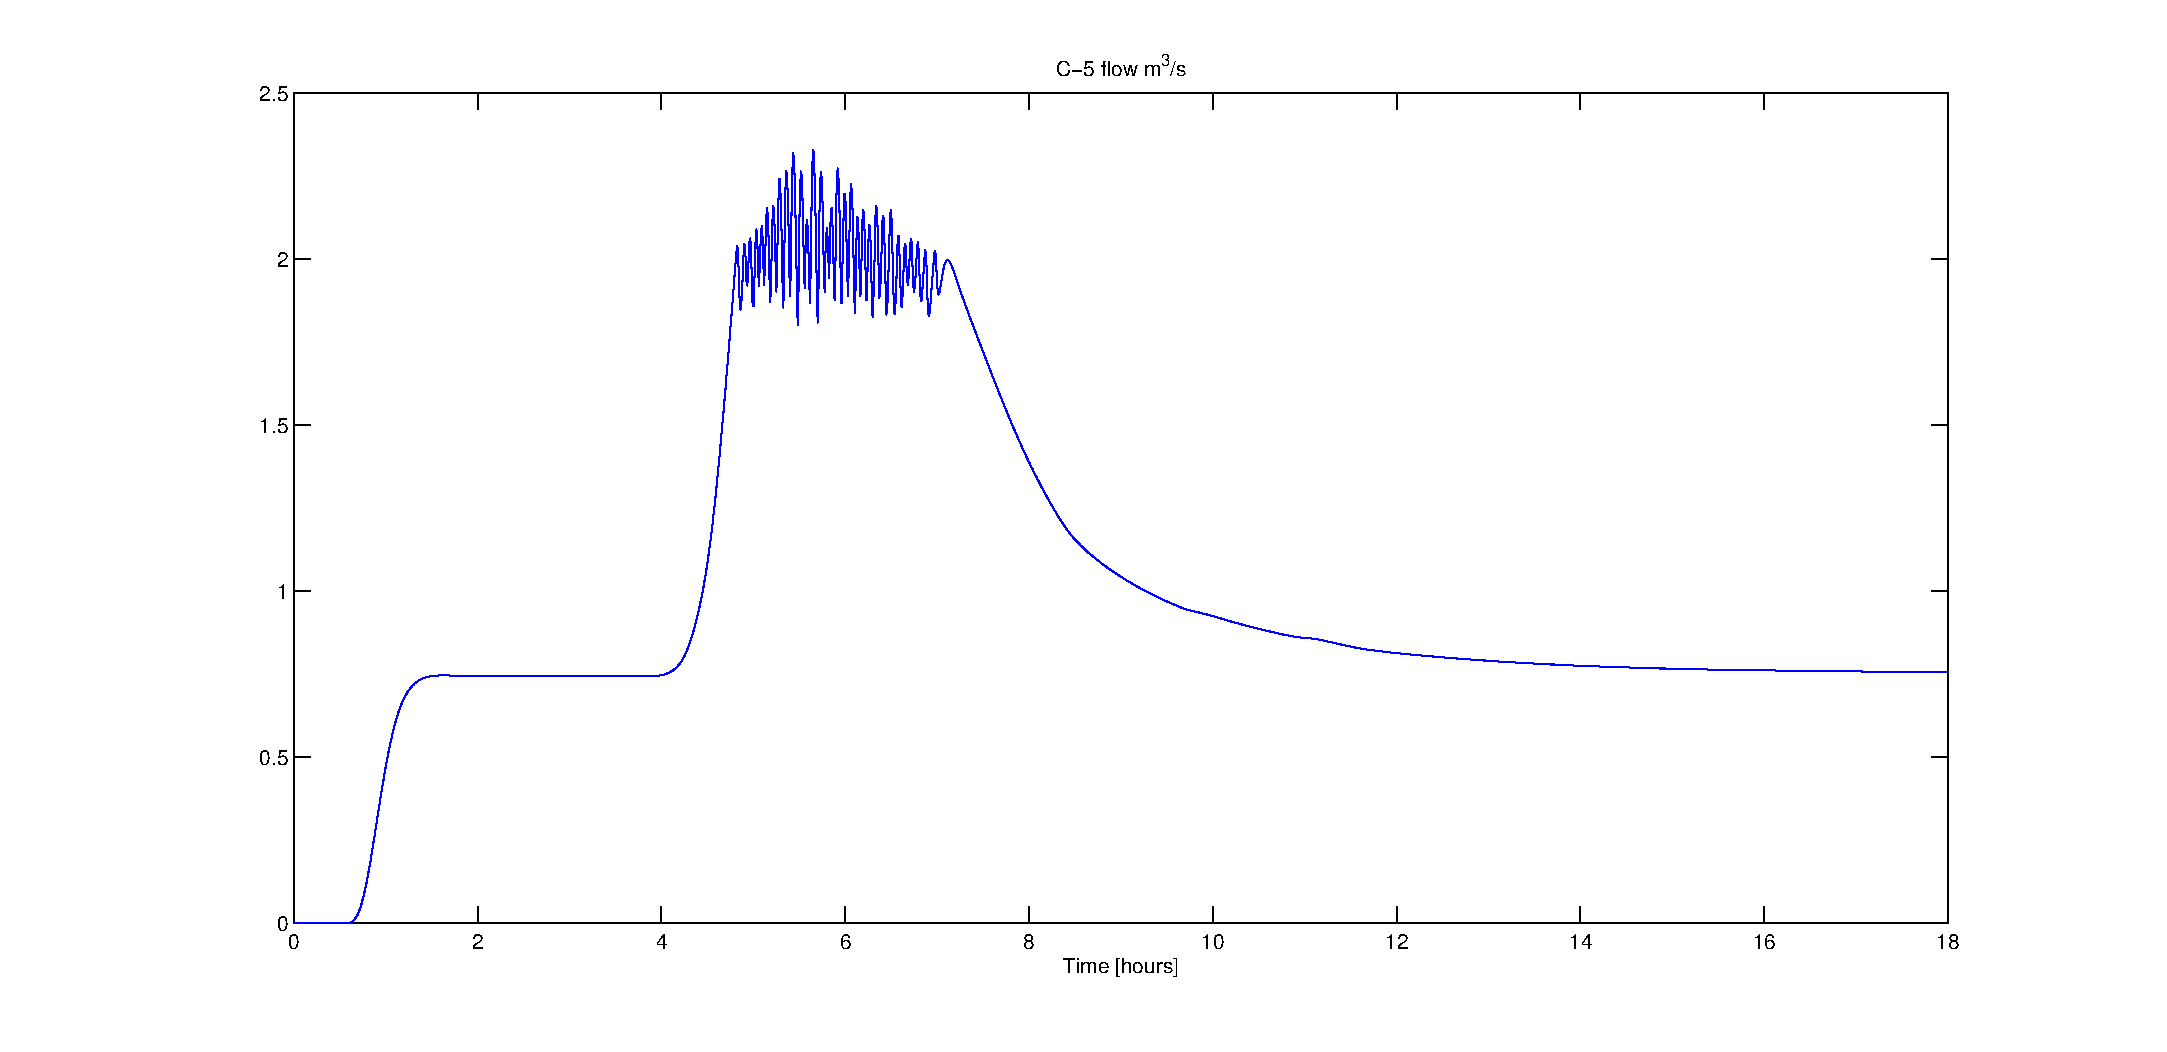
\includegraphics[height=7.5cm]{figs/matlab_1}
\caption{Matlab example results.}
\label{fig:matlab_ex}
\end{center}
\end{figure}

\subsection{The LabVIEW Toolbox}
\pagebreak

\section{Example running $n$ simulations}
\pagebreak
\end{document}